\chapter{Atchweliad Logistaidd}\label{cha:Atchweliad_logistaidd}
\section{Cefndir}
Defnyddiwn atchweliad logistaidd i fodelu'r tebygolrwydd o ddosbarthu gwrthrych i mewn i setiau deuaidd. Mae'n ddull o ddysgu dan oruchwyliaeth sy'n cael ei ddefnyddio yn aml yn academ\"{i}au a diwydiannau. Gall y atchweliad cael ei ddefnyddio i weld os mae rhywun yn curo/colli, s\^{a}l/iachus neu basio/methu mewn rhyw sefyllfa benodol. Gall y syniad yma cael ei ymestyn, gall wahanol atchweliadau logistaidd cael ei rhoi yn baralel i geisio rhoi'r tebygolrwydd o liw llygaid rhyw berson er enghraifft. Mewn termau mwy cyffredinol, gall ymestyn atchweliadau logistaidd i weithio ar setiau o labeli di-deuaidd. O hyn ymlaen fyddem yn edrych ar atchweliadau gyda labeli deuaidd\cite{logistic-regression}. 

Mae'n hawdd delweddu sut fydd atchweliad logistaidd gydag un newidyn annibynnol. Gwelwn fod y model yn edrych fel y graff yn Ddarlun~\ref{fig:Enghraifft_o_atchweliad_logistaidd} pan hyn yw'r sefyllfa.

\begin{figure}[H]
\begin{center}
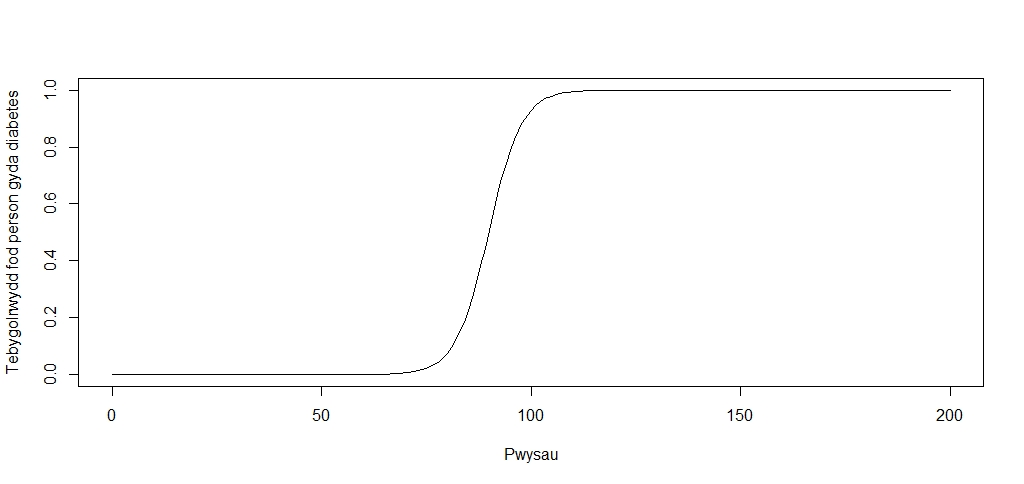
\includegraphics[width=0.5\linewidth]{../img/Atchweliad_logistaidd.jpeg}
\label{fig:Enghraifft_o_atchweliad_logistaidd}
\caption{Enghraiff o atchweliad logistaidd.}
\end{center}
\end{figure}

Gwelwn yn y graff nesaf fod y plot yn dangos ein data mewn ffordd rhesymol os wnawn gymharu i y cyfrannau o'r pwyntiau yn pob un o'r adrannau. Gwelwn y cyfrannau o phob adran yn wyrdd yn Ffigwr~\ref{fig:Enghraifft_o_atchweliad_logistaidd_pwyntiau_gyda_siart_bar}. 

\begin{figure}[H]
\begin{center}
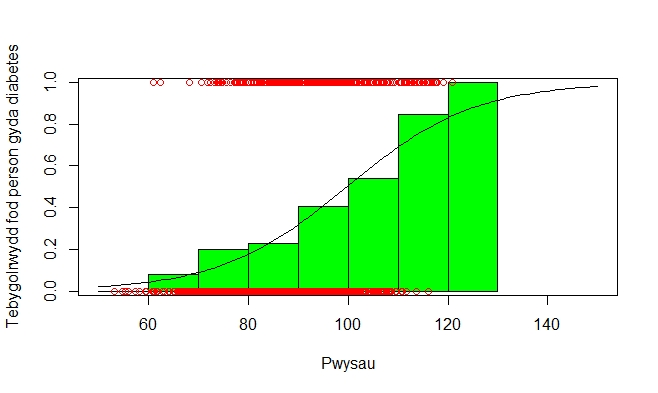
\includegraphics[width=0.5\linewidth]{../img/atchweliad_logistaidd_gyda_pwyntiau.jpeg}
\label{fig:Enghraifft_o_atchweliad_logistaidd_pwyntiau_gyda_siart_bar}
\caption{Enghraiff o atchweliad logistaidd gyda siart bar i ddangos cyfrannau o'r labeli.}
\end{center}
\end{figure}

Os wnawn cymharu y model logistaidd i model llinol, gwelwn yn y plot yn Darlun~\ref{fig:Enghraifft_o_atchweliad_llinol} dydy'r model ddim yn cynnal cynhaliad ar gyfer mewnbwn llai na $60$ a fwy na $120$ gan fod y tebygolrwydd yn anniffiniedig (Hynny yw, dydi ddim yn bosib cael $P(\mathbf{x})<0$ a $P(\mathbf{x})>1$). 

\begin{figure}[H]
\begin{center}
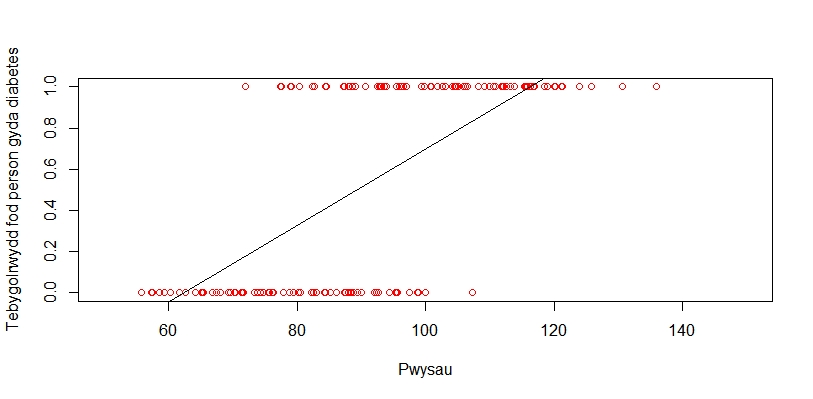
\includegraphics[width=0.5\linewidth]{../img/cymharu_llinol.jpeg}
\label{fig:Enghraifft_o_atchweliad_llinol}
\caption{Enghraiff o atchweliad llinol i ein data.}
\end{center}
\end{figure}

\section{Sut mae atchweliad logistaidd yn gweithio?}

Wnawn ddiffinio'r fector sy'n cynnwys gwybodaeth am berson $j$ ($j \in {1,\dots,n}$) gyda $\mathbf{x}_j$ sydd hefo dimensiwn o $m$ (hynny yw bod yna $m$ priodoleddau). Yn ogystal, wnawn ddiffinio $y_j$ fel label deuaidd i berson $j$, yr hyn rydyn ni eisiau rhagfynegi. Yna gydag ein data, gan ein bod yn perfformio dysgu dan oruchwyliaeth fyddwn yn hyfforddi'r algorithm yn defnyddio'r data hyfforddi ac yno yn gwirio'r algorithm drwy'r data profi. Felly wnawn hollti'r data fel:

Data hyfforddi: $\mathbf{x}_j$ a $y_j$ ar gyfer $j \in \{ 1,\dots,k\}$ lle mae $k<n$

Data profi: $\mathbf{x}_j$ a $y_j$ ar gyfer $j \in \{ k+1,\dots,n \}$

Mae'r model logistaidd yn cymryd y gwrthdro o ffurf logit, mae hyn yn cael ei ddangos yn Hafaliad~\ref{eqn:gwrthdrologit} lle mae $z \in (-\infty,\infty)$.

\begin{equation}\label{eqn:gwrthdrologit}	
	f(z) = \frac{1}{1+e^{-z}} 
\end{equation}

lle:

\begin{equation}\label{eqn:cyfernodau} 
    z = \alpha + \beta_{1}X_{1} + \dots + \beta_{m}X_{m} 
\end{equation} 

Felly mae hafaliad~~\ref{eqn:modellog} yn dangos y model cyfan.

\begin{equation}\label{eqn:modellog}
    P(\mathbf{x}) = P(y = 1 | x_1 \dots x_k) = \frac{1}{1+e^{-( \alpha + \sum_{i=1}^{m} \beta_{i}x_{i})}} 
\end{equation}

\subsection{Yr Algorithm}

Fydd $\alpha$ a $\mathbf{\beta}$ y paramedrau fyddem yn trio amcangyfrif o wybod $\mathbf{x}$ ac $y$ y data hyfforddi. I amcangyfrif hyn wnawn ddefnyddio'r dull amcangyfrif tebygoliaeth fwyaf. Cymerwn $\hat{\mathbf{z}}$ i fod y fector o baramedrau fyddem yn amcangyfrif. Yna mae gennym y amcangyfrif tebygoliaeth ganlynol a fyddem yn trio cael y gwerth agosaf i $1$. \cite{Logistic-regression}

\begin{equation}\label{eqn:amcangyfrif}
L(\hat{\mathbf{z}}) = \prod_{s \in y_{i}=1} p(x_i) \prod_{s \in y_{i}=0} (1 - p(x_i))
\end{equation}

Mae Hafaliad~\ref{eqn:amcangyfrif} yn trio uchafsymio y lluoswm o phob tebygolrwydd ag oedd yn edrych ar labeli y data hyfforddi. Gan fod rhai labeli am fod yn $0$ a lleill gyda $1$ ac rydym yn cymryd y lluoswm o'r rhifau gyda label o $0$ ag $1$, fydd y ddau luoswm ar wah\^{a}n yn cydgyfeirio am ddau werth gwahanol. Felly rydym yn dewis newid y lluoswm gyda labeli $0$ i gydgyfeirio tuag at $1$ drwy luosi'r lluoswm $1-p(x_i)$ i bob un gyda label $0$. Mae'n neud synnwyr cydgyfeirio i $1$ dros $0$ gan fod i gydgyfeirio tuag $0$ does dim ond angen un gwerth o $0$ yn y lluoswm. 

Sydd yn gallu cael ei symleiddio i:

$$ L(\hat{\mathbf{z}}) = \prod_{i=1}^{k} p(x_i)^{y_i} (1 - p(x_i))^{1-y_i} $$

Nawr fyddem yn cymryd y log o'r amcangyfrif tebygoliaeth.

$$ \log L(\hat{\mathbf{z}}) = \sum_{i=1}^{n} y_{i} \log(p(x_{i})) + (1-y_{i}) \log(1-p(x_{i})) $$

Sydd yn symleiddio i:

$$ \log L(\hat{\mathbf{z}}) = \sum_{i=1}^{n} y_{i} \log \left(\frac{1}{1 + e^{-\hat{\mathbf{z}}\mathbf{x}}} \right) + (1 - y_i) \log \left(\frac{e^{-\hat{\mathbf{z}}\mathbf{x}}}{1 + e^{-\hat{\mathbf{z}}\mathbf{x}}} \right) $$

ac felly:

$$ \log L(\hat{\mathbf{z}}) = \sum_{i=1}^{n} y_i \hat{\mathbf{z}} x_i - \log(1 + e^{\hat{\mathbf{z}} x_i}) $$

Yna mae gennym y log o'r amcangyfrif tebygoliaeth. Rydym eisiau darganfod y gwerth o $z$ lle mae'r log o'r amcangyfrif tebygoliaeth ar ei fwyaf.

$$ \hat{\mathbf{z}} = \arg \max_{\mathbf{z}} \log L(\mathbf{z})  $$

Does yna ddim ffordd bendant o ddatrys yr hafaliad uchod, fydd angen defnyddio algorithmau fel swm lleiaf sgwariau wedi eu hail-bwyso drwy iteriadau \cite{IWLS} neu algorithm cof-cyfengedig Broyden–Fletcher–Goldfarb–Shanno (BFGS) \cite{LBFGS} fel gwelwn yn y algorithmau yn R ac Python yn y drefn honno. Mae dull disgyniad fwyaf yn algorithm poblogaidd arall.

Mae'r dull disgyniad fwyaf yn algorithm optimeiddiaeth trefn cyntaf i darganfod isafbwynt lleol o ffwythiant gall ei ddifferu. Mae'r algorithm yn cymryd camau yn gyfraneddol i'r graddiant yn y pwynt yno. Fydd yr algorithm am phob cam yn edrych yn debyg i Hafaliad~\ref{eqn:disgyniadfwyaf} gyda $a$ yn rhyw bwynt a $f$ yn y ffwythiant.

\begin{equation}\label{eqn:disgyniadfwyaf}
  a_{n+1} = a_{n} - \nabla f
\end{equation}

Mae algorithm BFGS yn cychwyn gydag amcangyfrif cychwynnol o'r gwerth optimaidd $x_0$, ac yno yn iteru drwy ddefnyddio elfennau o matrics gwrthdro Hessian sef yr ail ddeilliad o'r ffwythiant. Mae'r Hessian yn cynnwys gwybodaeth bwysig am y crymedd.

Ar gyfer y swm lleiaf o sgwariau wedi eu hail-bwyso drwy iteriadau, mae'r algorithm yn cydgyfeirio tuag at y pwysau optimaidd ar gyfer y cyfernodau yn Hafaliad~\ref{eqn:cyfernodau}. Mae angen ail bwyso oherwydd mae'r amrywiant yn newid gydag $x$. Mae lle mae'r amrywiant ar ei fwyaf yn y model am dynodi lle fydd gromlin ein model.

\subsection{Profi'r model}

Unwaith mae gennym amcangyfrif o'r paramedrau, mae angen darganfod pa mor dda yw ein model logistaidd. I wneud hwn byddwn yn rhoi ein data profi $x_j$ i mewn i'r model, a cynharu'r allbwn gyda $y_j$. Fel allbwn cawn tebygolrywdd, rhif rhwng $0$ ac $1$, yna wnawn talgrynnu'r allbwn i cael label. Hynny yw os gawn ni allbwn llai na hanner, rhoddwn label $0$, fel arall bydd yn derbyn label $1$. Wedyn mae gennym ein rhagfynegiad am label pob person, yna gallwn ddarganfod cyfradd llwyddiant ein model gan:

\begin{equation}\label{eqn:cyfradd-llwyddiant}
 1 - \sum_{j = k+1}^{n} \frac{(P(\mathbf{x}_j) - y_j)^{2}}{n - k}
\end{equation}

Mae'r swm yma yn cymryd y canran o camgymeriadau rhwng y data hyfforddi a'r data profi ac yna yn ei tynnu i ffwrdd o $1$, byddwn yn menegi hwn fel y cyfradd llwyddiant. I darganfod y canran o camgymeriadau fyddwn yn tynnu y labeli y data profi oddi wrth labeli y data hyfforddi, ac yno yn sgwario yr fector canlyniadol. Fydd y gweithrediadau yma yn gweithio yn \^{o}l elfen. Unwaith fydd y fector wedi'i sgwario fydd pob elfen sy'n dangos $1$ yn dangos camgymeriad ac felly fydd $0$ yn dangos rhagfynegiad cywir. Yna fydd y fector yn cael ei symio ac fydd y cyfanswm yn cael ei rhannu gan y nifer o elfennau.

\section{Tiwtorial yn R}

Yn yr enghraifft hon, fyddwn yn edrych ar ddata ar 1000 o bobol, fydd y data yn cynnwys gwybodaeth ar taldra, pwysau, maint gwasg, oed, rhyw ag oes gan y person clefyd y siwgr. Mae'n bosib lawrlwytho'r data oddi: \url{https://dysgupeirianyddol.github.io/lawrlwythiadau/}

Ar gyfer gwneud atchweliad logistaidd, mae angen y pecyn \mintinline{R}{stats} a wnawn ei lawrlwytho a'i gosod gan redeg y canlynol:

\begin{minted}[bgcolor=green!7]{r}
> install.packages("stats")
> library(stats)
\end{minted}

Yna fydd rhaid lwytho'r data i mewn a'i arbed fel newidyn. Fydd rhaid neud yn si\^{w}r fod y ffwythiant \mintinline{R}{read.csv} yn cael ei chyfeirio tuag at y lleoliad cywir o le mae eich data chi wedi'i gadw.

\begin{minted}[bgcolor=green!7]{r}
> data <- read.csv("data_logistic.csv")
\end{minted}

Unwaith ei fod wedi llwytho, mae'n bosib gweld y data:

\begin{minted}[bgcolor=green!7]{r}
> View(data)
\end{minted}

\begin{figure}[H]
\begin{center}
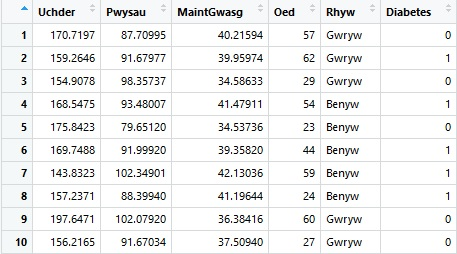
\includegraphics[width=0.5\linewidth]{../img/data_diabetes_r.jpg}
\end{center}
\end{figure}

Nawr wnawn rannu'r data fel bod $70\%$ o'r data yw'r data hyfforddi ac $30\%$ o'r data yw'r data profi. Fyddwn yn rhannu'r data ar hap. 

\begin{minted}[bgcolor=green!7]{r}
> rhifau <- c(1:1000)
> rhifauhyfforddi <- sample(x = rhifau, size = 700, replace = FALSE)
> rhifauprofi <- setdiff(rhifau, rhifauhyfforddi)
\end{minted}

Mae'r c\^{o}d uchod yn rhannu'r setiau gan ddefnyddio eu indecs (rhif y rhes) yn y data ac yno mae'r c\^{o}d isod yn rhannu'r fectorau i mewn i setiau arwahan. 

\begin{minted}[bgcolor=green!7]{r}
> hyfforddi <- data[rhifauhyfforddi,] 
> profi <- data[rhifauprofi,]
\end{minted}

Nawr rydym yn barod i greu'r model logistaidd. I greu'r model fyddem yn rhedeg y c\^{o}d gan ddefnyddio y ffwythiant \mintinline{R}{glm}, sydd yn fyr am "Generalized Linear Models", sydd yn golygu gall y ffwythiant cael ei ddefnyddio am lawer fwy o atchweliadau na logistaidd yn unig. Oherwydd hyn mae angen gosod yr opsiwn \mintinline{R}{family} i \mintinline{R}{binomial}. I ddilyn strwythur o'r algorithm, byddwn yn creu'r model o'r data hyfforddi yn unig. 

\begin{minted}[bgcolor=green!7]{r}
> atchweliad <- glm(Clefyd_Siwgr ~ Taldra + Pwysau + Oed + Rhyw + MaintGwasg,
+                   family = binomial,
+                   data = hyfforddi)
\end{minted}

Unwaith mae'r model wedi'i greu, gallwn weld eu paramedrau sydd wedi cael ei amcangyfrif:

\begin{minted}[bgcolor=green!7]{r}
> atchweliad$coefficients
 (Intercept)       Taldra       Pwysau          Oed 
22.858432583 -0.254347133  0.215272873  0.057360113 
   RhywGwryw   MaintGwasg 
-8.074052403 -0.003206262 
\end{minted}

Felly mae'r model sydd gennym, i dri lle degl, yn edrych fel:

$$ P(\mathbf{x}) = \frac{1}{1 + e^{-22.858 + 0.254 x_{\text{Taldra}} - 0.215 x_{\text{Pwysau}} - 0.057 x_{\text{Oed}} + 8.074 x_{\text{Rhyw}} + 0.003 x_{\text{MaintGwasg}}}} $$

Gan fod ein model wedi'i chwblhau, gallwn weld sut mae'n perfformio yn penderfynu os oes gan bobl y set profi clefyd siwgr neu peidio. Geith hyn ei wneud yn defnyddio'r ffwythiant \mintinline{R}{predict} a dewis yr opsiwn \mintinline{R}{type} fel \mintinline{R}{response} i gael allbwn o debygolrwydd. Heb wneud hyn, fydd yr allbwn yn cyfrifo $z$ o Hafaliad~\ref{eqn:cyfernodau}. 

\begin{minted}[bgcolor=green!7]{r}
> canlyniad <- predict(object = atchweliad, newdata = profi, type = "response")
> canlyniad <- round(canlyniad, digits = 0)
> canlyniad <- unname(canlyniad)
\end{minted}

Fyddem yn ogystal yn talgrynnu'r tebygolrwydd o bob person i cael dewis ar os gennym clefyd siwgr neu peidio. Wedyn fyddem yn tynnu i ffwrdd y rhifau o'r rhesi ar y fector o labeli. Nawr gennym y rhagfynegiad a'r canlyniadau gwreiddiol, gallwn gyfrifo'r canran o'r ddau set sy'n debyg. Gallwn gyfrifo yn y ffurf ganlynol gan fod ein setiau yn ddeuaidd:

\begin{minted}[bgcolor=green!7]{r}
> 1-(sum((test[,6]-unname(canlyniad))**2)/length(test[,6]))
0.8833333
\end{minted}

Fel y gwelwn, mae ein model gyda cywirdeb o $88\%$ ar gyfer y data sydd gennym. Gallwn ni defnyddio y model rydym wedi creu i benderfynu ar os gan berson newydd ar hap clefyd siwgr neu ddim. Gwelwn hyn gan gyflwyno dyn gydag Taldra o 160, pwysau 92, maint gwasg o 34 ag ugain oed yn y c\^{o}d isod: 

\begin{minted}[bgcolor=green!7]{r}
> unname(round(predict(object = atchweliad, 
+                      newdata = data.frame(Taldra = 160,
+                                           Pwysau = 92, 
+                                           MaintGwasg = 34, 
+                                           Oed = 20, 
+                                           Rhyw = "Gwryw"), 
+                      type = "response"),
+              digits = 0))
+ 
0
\end{minted}

Am y person yma gwelwn fod y model wedi rhagfynegu nad oes ganddo clefyd siwgr. Os wnawn ystyried person gyda'r un nodweddion ond yn fenyw:

\begin{minted}[bgcolor=green!7]{r}
> unname(round(predict(object = atchweliad,
+                      newdata = data.frame(Taldra = 160,
+                                           Pwysau = 92, 
+                                           MaintGwasg = 34, 
+                                           Oed = 20, 
+                                           Rhyw = "Benyw"), 
+                      type = "response"),
+              digits = 0))
+ 
1
\end{minted}

Gwelwn fod y model yn rhagfynegi ei fod hi gyda clefyd siwgr.

\section{Tiwtorial yn Python}

Ar gyfer cynhyrchu atchweliad logistaidd yn python mae rhaid i ni ddefnyddio'r pecynnau \mintinline{python}{sklearn}, a \mintinline{python}{pandas} i trin y data. Wnawn lwytho'r pecynnau gan redeg y c\^{o}d yma:

\begin{minted}[bgcolor=cyan!7]{python}
>>> from sklearn.linear_model import LogisticRegression
>>> import pandas as pd
\end{minted}

Nawr mae angen llwytho'r data, wnawn ddefnyddio data sy'n cynnwys 1000 o gofnodion data ar fesuriadau pobl yn cynnwys taldra, pwysau, maint gwasg, oed, rhyw ag oes gan y person clefyd y siwgr. Cewch ei lawrlwytho o \url{https://dysgupeirianyddol.github.io/lawrlwythiadau/}.

\begin{minted}[bgcolor=cyan!7]{python}
>>> data = pd.read_csv('data_logistic.csv')
\end{minted}

Gallwn gweld yr data gan rhedeg:

\begin{minted}[bgcolor=cyan!7]{python}
>>> data.head()
\end{minted}

\begin{figure}[H]
\begin{center}
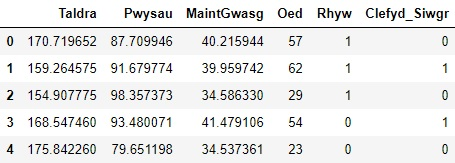
\includegraphics[width=0.5\linewidth]{../img/data_diabetes_python.jpg}
\end{center}
\end{figure}

Gan fod ein data gyda rhyw wedi cael ei diffinio gyda'r geiriau ``Gwryw'' a ``Benyw'', mae Python yn cael trafferth yn delio gyda nhw. Felly nawn trawsnewid nhw i newidyn deuaidd (set o $1$ a $0$).

\begin{minted}[bgcolor=cyan!7]{python}
>>> data['Rhyw'] = data['Rhyw'].apply(lambda x: int(x =='Gwryw'))
\end{minted}

Nawr fydd rhaid i ni rannu'r data i ddata hyfforddi ag data profi.

\begin{minted}[bgcolor=cyan!7]{python}
>>> hyfforddi = data.sample(frac = 0.7)
>>> profi = data.drop(hyfforddi.index)
\end{minted}

Mae'r wybodaeth rydym angen i greu model logistaidd angen fod yn fatrics yn Python, felly:

\begin{minted}[bgcolor=cyan!7]{python}
>>> X = hyfforddi[['Taldra', 'Pwysau', 'MaintGwasg', 'Oed', 'Rhyw']].as_matrix()
>>> y = hyfforddi['Clefyd_Siwgr'].as_matrix()
>>> X_profi = profi[['Taldra', 'Pwysau', 'MaintGwasg', 'Oed', 'Rhyw']].as_matrix()
>>> y_profi = profi['Clefyd_Siwgr'].as_matrix()
\end{minted}

I redeg yr atchweliad logistaidd wnawn ddefnyddio'r ffwythiant yn \mintinline{python}{sklearn}. Wnawn wneud gan redeg y c\^{o}d canlynol:

\begin{minted}[bgcolor=cyan!7]{python}
>>> clf = LogisticRegression(random_state=0).fit(X, y)
\end{minted}

Gallwn edrych ar y rhyngdoriad gan

\begin{minted}[bgcolor=cyan!7]{python}
>>> clf.intercept_
array([ 1.70933553])
\end{minted}

ac yna y paramedrau eraill:

\begin{minted}[bgcolor=cyan!7]{python}
>>> clf.coef_
array([[-0.12384414,  0.14710498,  0.12995053,  0.04682347, -4.80795833]])
\end{minted}

Felly dyma yw ein model i dri lle degol:

$$ P(\mathbf{x}) = \frac{1}{1 + e^{-1.709 + 0.124 x_{\text{Taldra}} + 0.147 x_{\text{Pwysau}} - 0.047 x_{\text{Oed}} + 4.808 x_{\text{Rhyw}} - 0.130 x_{\text{MaintGwasg}}}} $$

Nawr gallwn ni cyfrifo'r gyfradd llwyddiant o ein model ar y data profi. Gallwn ei chyfrifo yn y ffordd ganlynol oherwydd ein bod yn delio gyda data deuaidd.

\begin{minted}[bgcolor=cyan!7]{python}
>>> 1-(sum((clf.predict(X_profi)-y_profi)**2)/len(y_profi))
0.91666666666666663
\end{minted}

Felly mae ein model logistaidd yn python yn rhoi cyfradd llwyddiant o tua $92\%$. Gallwn nawr ei ddefnyddio ar gyfer rhyw berson tu allan i ein data. Os oes gennym wryw gyda thaldra o 171, pwysau o 130 a maint gwasg ag oed o 40; gallwn ragfynegi os oes gan y person clefyd siwgr ta ddim. 

\begin{minted}[bgcolor=cyan!7]{python}
>>> clf.predict([[171, 130, 40, 40, 1]])
array([1], dtype=int64)
\end{minted}

Gwelwn fod y model logistaidd yn rhagfynegu bod gan y person hwn clefyd siwgr. Nawr nawn drio gyda person tebyg ond gyda phwysau o 90 yn lle.

\begin{minted}[bgcolor=cyan!7]{python}
>>> clf.predict([[171, 90, 40, 40,1]])
array([0], dtype=int64)
\end{minted}

Gwelwn nad oes gan y person yma clefyd siwgr.